
\begin{itemize}
   \item ¿Cómo recupera un motor de búsqueda, como Duckduckgo o Google, los documentos relevantes a partir de una consulta dada?
   \item ¿Cómo puede una empresa procesar las reclamaciones dejadas por sus usuarios en sus portales web?
\end{itemize}

Estos problemas se estudian en los siguientes campos:

\begin{itemize}
   \item \emph{Recuperación de Información}: ciencia de buscar información en colecciones de documentos.
   \item \emph{Minería de Texto}: extracción automática de conocimiento a partir de texto.
\end{itemize}

¡Ambos están estrechamente relacionados con el Procesamiento del Lenguaje Natural (NLP, por sus siglas en inglés)! (las fronteras entre estos campos no están claras).

\section{Tokens y Tipos}

Tokenización: la tarea de dividir una oración o documento en fragmentos llamados \emph{tokens}. \\
Se pueden emplear transformaciones adicionales, como la eliminación de caracteres especiales (por ejemplo, puntuación), minúsculas, etc. ~\cite{manning2008}.

\paragraph{Ejemplo}
Entrada: Me gustan los lenguajes humanos y los lenguajes de programación.\\
Tokens: [Me] [gustan] [los] [lenguajes] [humanos] [y] [los] [lenguajes] [de] [programación]


\paragraph{Tipos}
\begin{itemize}
\item Un \emph{tipo} es una clase de \emph{token} que contiene una única secuencia de caracteres.
\item Se obtienen identificando los tokens únicos dentro del documento.
\end{itemize}

Tipos para la oración anterior: [Me] [gustan] [los] [lenguajes] [humanos] [y] [de] [programación] \
El token \emph{lenguajes} se repitió en la oración.

\paragraph{Extracción de Vocabulario}

\begin{itemize}
\item Un \emph{término} es un \emph{tipo} normalizado.
\item La normalización es el proceso de crear clases de equivalencia de diferentes \emph{tipos}. Esto quedará claro en las siguientes diapositivas.
\item El vocabulario $V$ es el conjunto de términos (tokens únicos normalizados) dentro de una colección de documentos o corpus $D$.
\end{itemize}

\paragraph{Eliminación de stopwords}
\begin{itemize}
\item Con el fin de reducir el tamaño del vocabulario y eliminar términos que no aportan mucha información, se eliminan los términos que ocurren con alta frecuencia en el corpus.
\item Estos términos se llaman \emph{stopwords} e incluyen artículos, pronombres, preposiciones y conjunciones. \
Ejemplo: [un, una, y, cualquier, tiene, hacer, no, hizo, el, en].
\end{itemize}

¡La eliminación de stopwords puede ser inconveniente en muchas tareas de procesamiento del lenguaje natural!

Ejemplo: No me gusta la pizza $=>$ pizza (se eliminaron "no", "me" y "gusta")

\paragraph{Stemming}

Es un proceso de normalización de términos en el cual los términos se transforman a su raíz con el objetivo de reducir el tamaño del vocabulario. Se lleva a cabo aplicando reglas de reducción de palabras. \
Ejemplo: Algoritmo de Porter.

\begin{figure}[h!]
\centering
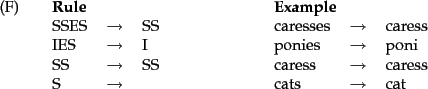
\includegraphics[scale=0.45]{pics/porter.png}
\end{figure}

Ejemplo: $d$ = Me gustan los lenguajes humanos y los lenguajes de programación $=>$ Me gustan los lenguaj y los program lenguaj\footnote{\url{http://9ol.es/porter_js_demo.html}}

El vocabulario del documento $d$ después de eliminar stopwords y realizar stemming:

\begin{table}
\centering
\begin{tabular}{c|c}
\hline
termId & value \\
\hline
t1 & human \\
t2 & languag \\
t3 & program\\
\hline
\end{tabular}
\end{table}


\paragraph{Lematización}

\begin{itemize}
   \item Otra estrategia de normalización de términos.
   \item También transforma las palabras en sus raíces.
   \item Realiza un análisis morfológico utilizando diccionarios de referencia (tablas de búsqueda) para crear clases de equivalencia entre \emph{tipos}.
   \item Por ejemplo, para el token \emph{estudios}, una regla de stemming devolvería el término \emph{estudi}, mientras que a través de la lematización obtendríamos el término \emph{study}\footnote{\url{https://blog.bitext.com/what-is-the-difference-between-stemming-and-lemmatization/}}.
\end{itemize}

\subsection{Ley de Zipf}
\begin{itemize}
   \item La Ley de Zipf, propuesta por \emph{George Kingsley Zipf} en \cite{zipf1935}, es una ley empírica sobre la frecuencia de los términos dentro de una colección de documentos (\textbf{corpus}).
   \item Establece que la frecuencia $f$ de un término en un corpus es inversamente proporcional a su posición $r$ en una tabla de frecuencia ordenada:
   \begin{equation}
      f = \frac{cf}{r^{\beta}}
   \end{equation}
   \item Donde $cf$ es una constante dependiente de la colección y $\beta > 0$ es un factor de decaimiento.
   \item Si $\beta = 1$, entonces $f$ sigue exactamente la Ley de Zipf; de lo contrario, sigue una distribución similar a la de Zipf.
   \item La ley se relaciona con el principio del mínimo esfuerzo. A menudo utilizamos pocas palabras para expresar ideas.
   \item La Ley de Zipf es un tipo de distribución de ley de potencia (distribuciones de cola larga).
\end{itemize}

\begin{figure}[h!]
	\centering
	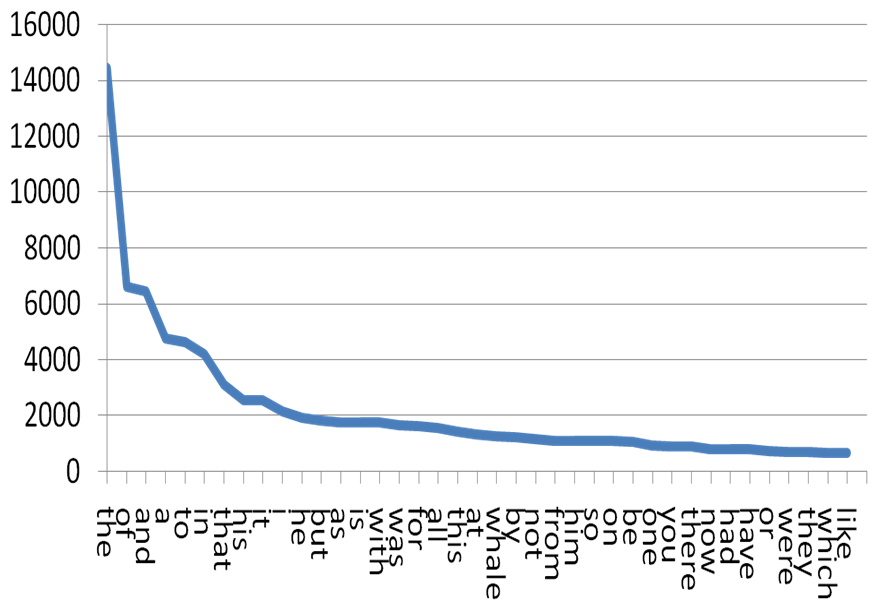
\includegraphics[scale=0.5]{pics/zipf1.png}
	\caption{Ley de Zipf}
\end{figure}

\begin{itemize}
   \item Si trazamos un gráfico de $log$-$log$, obtenemos una línea recta con una pendiente de $-\beta$.
   \item Enumerar las palabras más frecuentes de un corpus se puede utilizar para construir una lista de \emph{stopwords}.
\end{itemize}
\subsection{Listas de publicaciones y el índice invertido}
Sea $D$ una colección de documentos y $V$ el vocabulario de todos los términos extraídos de la colección:

\begin{itemize}
\item La lista de publicaciones de un término es la lista de todos los documentos donde el término aparece al menos una vez. Los documentos se identifican por sus identificadores.
\item Un índice invertido es una estructura de datos tipo diccionario que mapea los términos $t_{i} \in V$ con sus listas de publicaciones correspondientes.
\begin{displaymath}
<\text{término}> \rightarrow <\text{idDocumento}>^*
\end{displaymath}
\end{itemize}

\begin{figure}[h!]
\centering
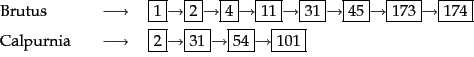
\includegraphics[scale=0.6]{pics/invFile.png}
\caption{Índice invertido}
\end{figure}

\subsection{Motores de búsqueda web}

Un motor de búsqueda es un sistema de recuperación de información diseñado para buscar información en la web (satisfacer necesidades de información) \cite{manning2008}. Sus componentes básicos son:

\begin{itemize}
\item Rastreador: un robot que navega por la web según una estrategia definida. Por lo general, comienza navegando por un conjunto de sitios web iniciales y continúa navegando a través de sus enlaces.
\item Indexador: se encarga de mantener un índice invertido con el contenido de las páginas recorridas por el rastreador.
\item Procesador de consultas: se encarga de procesar las consultas de los usuarios y buscar en el índice los documentos más relevantes para una consulta.
\item Función de clasificación: la función utilizada por el procesador de consultas para clasificar los documentos indexados en la colección por relevancia según una consulta.
\item Interfaz de usuario: recibe la consulta como entrada y devuelve los documentos clasificados por relevancia.
\end{itemize}

\begin{figure}[h!]
\centering
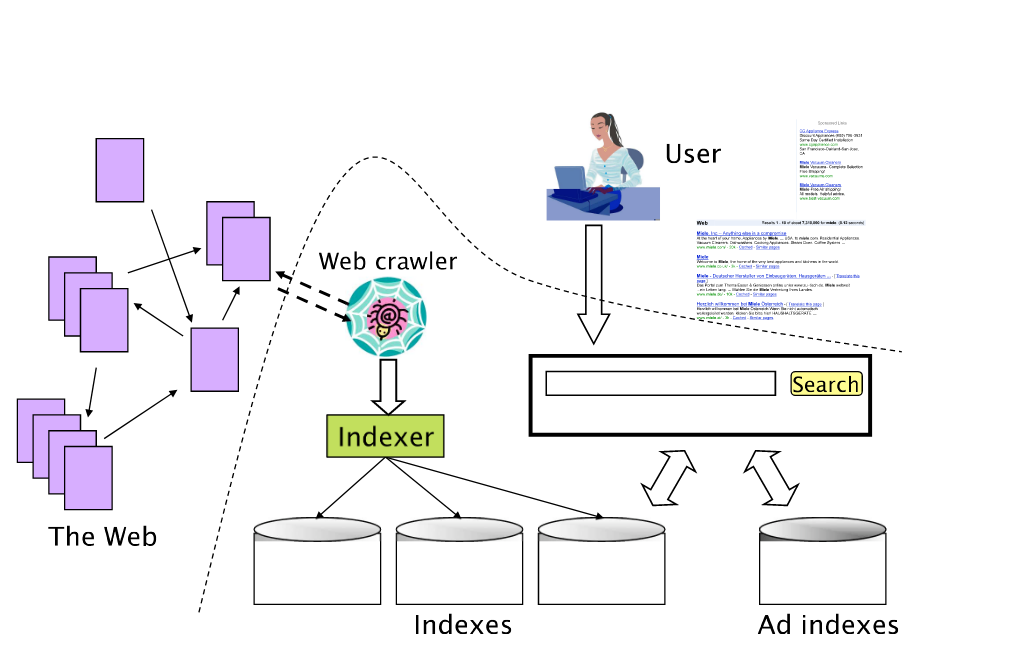
\includegraphics[scale=0.25]{pics/searchengine.png}
\caption{Los diversos componentes de un motor de búsqueda web \cite{manning2008}.}
\end{figure}
\section{El modelo de espacio vectorial}

\begin{itemize}
\item Para clasificar consultas o medir la similitud entre dos documentos, necesitamos una métrica de similitud.
\item Los documentos pueden ser \textit{representados} como vectores de términos, donde cada término es una dimensión del vector \cite{salton1975vector}.
\item Documentos con diferentes palabras y longitudes residirán en el mismo espacio vectorial.
\item Este tipo de representaciones se llaman \emph{Bolsa de Palabras} (Bag of Words).
\item En las representaciones de bolsa de palabras, se pierde el orden de las palabras y la estructura lingüística de una oración.
\item El valor de cada dimensión es un peso que representa la relevancia del término $t_{i}$ en el documento $d$.
\begin{equation}
d_{j} \rightarrow \overrightarrow{d_{j}}=(w(t_{1},d_{j}),...,w(t_{|V|},d_{j}))
\end{equation}
\item ¿Cómo podemos modelar la información que aporta un término a un documento?
\end{itemize}

\paragraph{Frecuencia de Término - Frecuencia Inversa de Documento}

\begin{itemize}
\item Sea $tf_{i,j}$ la frecuencia del término $t_{i}$ en el documento $d_{j}$.
\item Un término que ocurre 10 veces debería proporcionar más información que uno que ocurre solo una vez.
\item ¿Qué ocurre cuando tenemos documentos que son mucho más largos que otros?
\item Podemos normalizar dividiendo por la frecuencia máxima del término en el documento.
\begin{displaymath}
ntf_{i,j}=\frac{tf_{i,j}}{\max_i (tf_{i,j})}
\end{displaymath}
\item ¿Un término que ocurre en muy pocos documentos proporciona más o menos información que uno que ocurre varias veces?
\item Por ejemplo, el documento \emph{El respetado alcalde de Pelotillehue}. El término \emph{Pelotillehue} ocurre en menos documentos que el término \emph{alcalde}, por lo que debería ser más descriptivo.
\item Sea $N$ el número de documentos en la colección y $n_{i}$ el número de documentos que contienen el término $t_{i}$, definimos la frecuencia inversa de documento ($idf$) de $t_{i}$ de la siguiente manera:
\begin{displaymath}
idf_{t_{i}}= \log_{10}\left(\frac{N}{n_{i}}\right)
\end{displaymath}
\item Un término que aparece en todos los documentos tendría $idf=0$, y uno que aparece en el $10\%$ de los documentos tendría $idf=1$.
\item El modelo de puntuación $tf$-$idf$ combina las puntuaciones de $tf$ e $idf$, y resulta en los siguientes pesos $w$ para un término en un documento:
\begin{displaymath}
w(t_{i},d_{j})=tf_{i}\times \log_{10}\left(\frac{N}{n_{i}}\right)
\end{displaymath}
\item Las consultas de los motores de búsqueda también pueden ser modeladas como vectores. Sin embargo, en promedio, las consultas suelen tener entre 2 y 3 términos. Para evitar tener demasiadas dimensiones nulas, los vectores de consulta pueden suavizarse de la siguiente manera:
\begin{displaymath}
w(t_{i},d_{j})=(0.5+0.5\times tf_{i,j})\log_{10}\left(\frac{N}{n_{i}}\right)
\end{displaymath}
\end{itemize}

\subsection{Similitud entre vectores}
\begin{itemize}
\item Representar consultas y documentos como vectores permite calcular su similitud.
\item Un enfoque podría ser utilizar la distancia euclidiana.
\item El enfoque común es calcular el coseno del ángulo entre los dos vectores.
\item Si ambos documentos son iguales, el ángulo sería $0$ y su coseno sería $1$. Por otro lado, si son ortogonales, el coseno es $0$.
\item La similitud del coseno se calcula de la siguiente manera:
\begin{displaymath}
\text{similitud del coseno}(\vec{d}{1},\vec{d}{2})= \frac{\vec{d}{1}\cdot \vec{d}{2}}{|\vec{d}{1}|\times|\vec{d}{2}|} = \frac{\sum_{i=1}^{|V|}(w(t_{i},d_{1})\times w(t_{i},d_{2}))}{\sqrt{\sum_{i=1}^{|V|} w(t_{i},d_{1})^2}\times \sqrt{\sum_{i=1}^{|V|} w(t_{i},d_{2})^2}}
\end{displaymath}
\item Esto se llama incorrectamente "distancia del coseno". En realidad, es una métrica de similitud.
\item Observa que la similitud del coseno normaliza los vectores por su norma euclidiana $||\vec{d}||_{2}$.

\end{itemize}

\begin{figure}[h!]
\centering
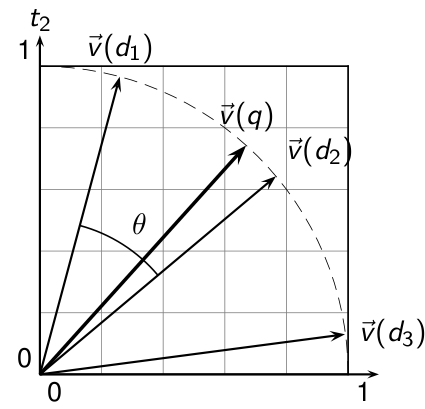
\includegraphics[scale=0.5]{pics/cos.png}
\caption{Similitud del coseno.}
\end{figure}
\paragraph{Ejercicio}
\begin{itemize}
\item Supongamos que tenemos $3$ documentos formados a partir de las siguientes secuencias de términos: \
$d_{1}\rightarrow t_{4}t_{3}t_{1}t_{4}$ \
$d_{2}\rightarrow t_{5}t_{4}t_{2}t_{3}t_{5}$ \
$d_{3}\rightarrow t_{2}t_{1}t_{4}t_{4}$ \
\item Construye una matriz término-documento de dimensiones $5\times3$ utilizando pesos simples de $tf$-$idf$ (sin normalización).
\item Recomendamos que primero construyas una lista con el número de documentos en los que aparece cada término (útil para calcular los valores de $idf$).
\item Luego, calcula los valores de $idf$ para cada término.
\item Rellena las celdas de la matriz con los valores de $tf$-$idf$.
\item ¿Cuál es el documento más cercano a $d_{1}$?
\end{itemize}

 \begin{table}[htbp]
 \centering
\begin{tabular}{|l|r|r|r|}
\hline
 & \multicolumn{1}{l|}{d1} & \multicolumn{1}{l|}{d2} & \multicolumn{1}{l|}{d3} \\ \hline
t1 & 0.176 & 0.000 & 0.176 \\ \hline
t2 & 0.000 & 0.176 & 0.176 \\ \hline
t3 & 0.176 & 0.176 & 0.000 \\ \hline
t4 & 0.000 & 0.000 & 0.000 \\ \hline
t5 & 0.000 & 0.954 & 0.000 \\ \hline
\end{tabular}
\caption{Matriz tf-idf}
\end{table}

\section{Agrupamiento de Documentos}

\begin{itemize}
\item ¿Cómo podemos agrupar documentos que son similares entre sí?
\item El agrupamiento es el proceso de agrupar documentos que son similares entre sí.
\item Cada grupo de documentos se llama \emph{cluster} o grupo.
\item En el agrupamiento, intentamos identificar grupos de documentos en los que la similitud entre documentos en el mismo grupo se maximiza y la similitud de documentos en diferentes grupos se minimiza.
\begin{figure}[h!]
\centering
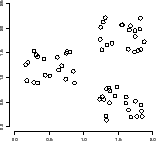
\includegraphics[scale=0.6]{pics/cluster.png}
\caption{ Conjunto de documentos donde los grupos se pueden identificar claramente.}
\end{figure}
\item El agrupamiento de documentos permite identificar temas en un corpus y reducir el espacio de búsqueda en un motor de búsqueda, es decir, el índice invertido se organiza según los grupos.
\item K-means es un algoritmo de agrupamiento simple que recibe el número de grupos $k$ como parámetro.
\item El algoritmo se basa en la idea de \emph{centroide}, que es el vector promedio de los documentos que pertenecen al mismo grupo.
\item Sea $S$ un conjunto de vectores bidimensionales ${3,6}, {1,2}, {5,1}$, el centroide de $S$ es ${(3+1+5)/3,(6+2+1)/3} = {3,3}$.

\end{itemize}

\subsection{K-Means}
\begin{enumerate}
\item Comenzamos con $k$ centroides aleatorios.
\item Calculamos la similitud entre cada documento y cada centroide.
\item Asignamos cada documento a su centroide más cercano formando un grupo.
\item Se recalculan los centroides de acuerdo a los documentos asignados a ellos.
\item Este proceso se repite hasta la convergencia.
\end{enumerate}

\begin{figure}[h!]
\centering
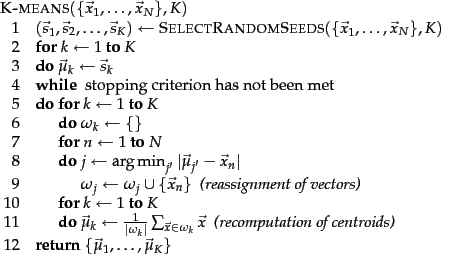
\includegraphics[scale=0.6]{pics/kmeans.png}
\caption{ Algoritmo K-means}
\end{figure}

\section{Conclusiones y Conceptos Adicionales}
\begin{itemize}
\item Representar documentos como vectores es fundamental para calcular similitudes entre pares de documentos.
\item Los vectores de "bag of words" carecen de estructura lingüística.
\item Los vectores de "bag of words" son de alta dimensionalidad y dispersos.
\item Los n-gramas de palabras pueden ayudar a capturar expresiones de múltiples palabras (por ejemplo, New York $=>$ new\_york)
\item Los sistemas modernos de recuperación de información van más allá de la similitud de vectores (PageRank, Retroalimentación de relevancia, Minería de registros de consultas, Grafo de conocimiento de Google, Aprendizaje automático).
\item La recuperación de información y la minería de textos se preocupan menos por la estructura lingüística y más por producir algoritmos rápidos y escalables \cite{jacobbook}.
\end{itemize}
